The overall design of this project can be split into three phases:

\begin{enumerate}
    \item Residue identity prediction: in this phase, we train two equivariant GNN models on the RES task, using the ATOM 3D dataset \cite{atom-3d}.
    \item Mutation generation: in this phase, we repurpose the models trained in Phase 1 to generate possible amino-acid mutations for a subset of proteins from the ProteinGym dataset \cite{tranception}; we then evaluate how much better these mutations are than the wildtype (base protein). 
    \item Protein fitness prediction: in the last phase, we use the models trained in Phase 1 to generate position scores for every possible amino-acid in a sequence. We use these scores as features in a ridge regression model in order to score the fitness of each single-point mutation in the ProteinGym dataset \cite{tranception}.
\end{enumerate}

\section{Residue identity prediction}
The Residue Identity (RES) task focuses on the prediction of amino acid identities within a protein's structural environment. Specifically, our objective is to accurately classify the amino acid present at a given site based on the surrounding atoms. To address this task, we use the ATOM3D dataset \cite{atom-3d}, comprising of atomic environments extracted from non-redundant structures in the Protein Data Bank (PDB). This dataset serves as the foundation for formulating the RES task as a classification problem. 

\subsection{Dataset details}
One of the standard formats for representing protein structure is the Protein Data Bank format (PDB). This text-based format contains information about all of the levels of protein's structure (i.e., primary, secondary, and tertiary). For the tertiary structure, the file describes the 3D coordinates of the atoms in the protein. Each atom record includes information such as the atom name, atom type, residue name, residue number, and the X, Y, and Z coordinates. Table \ref{dataset_stats} provides a summary of the statistics of the full RES ATOM3D dataset.

\paragraph{Local environments.} For each molecule in the dataset, the creators provide samples of local atomic environments. Each sample indicates the indices of the atoms to select from the original PDB file, as well as the target amino-acid.
We use these samples to generate masked local environments to feed into the ML model. Figure \ref{protein_pipeline} illustrates this pipeline conceptually. 

\paragraph{Side-chain masking.} As mentioned in Section \ref{amino-acids}, all amino-acid residues share the same underlying \textit{backbone} structure. Due to this reason, when masking the target amino-acid, the authors of the RES dataset only remove its \textit{side-chain} atoms. The side-chain is always bound to the $\text{C}_{\alpha}$ atom of the residue, so we train the ML model to classify this atom as one of the 20 naturally occurring amino-acids.


\begin{figure}
    \centering
    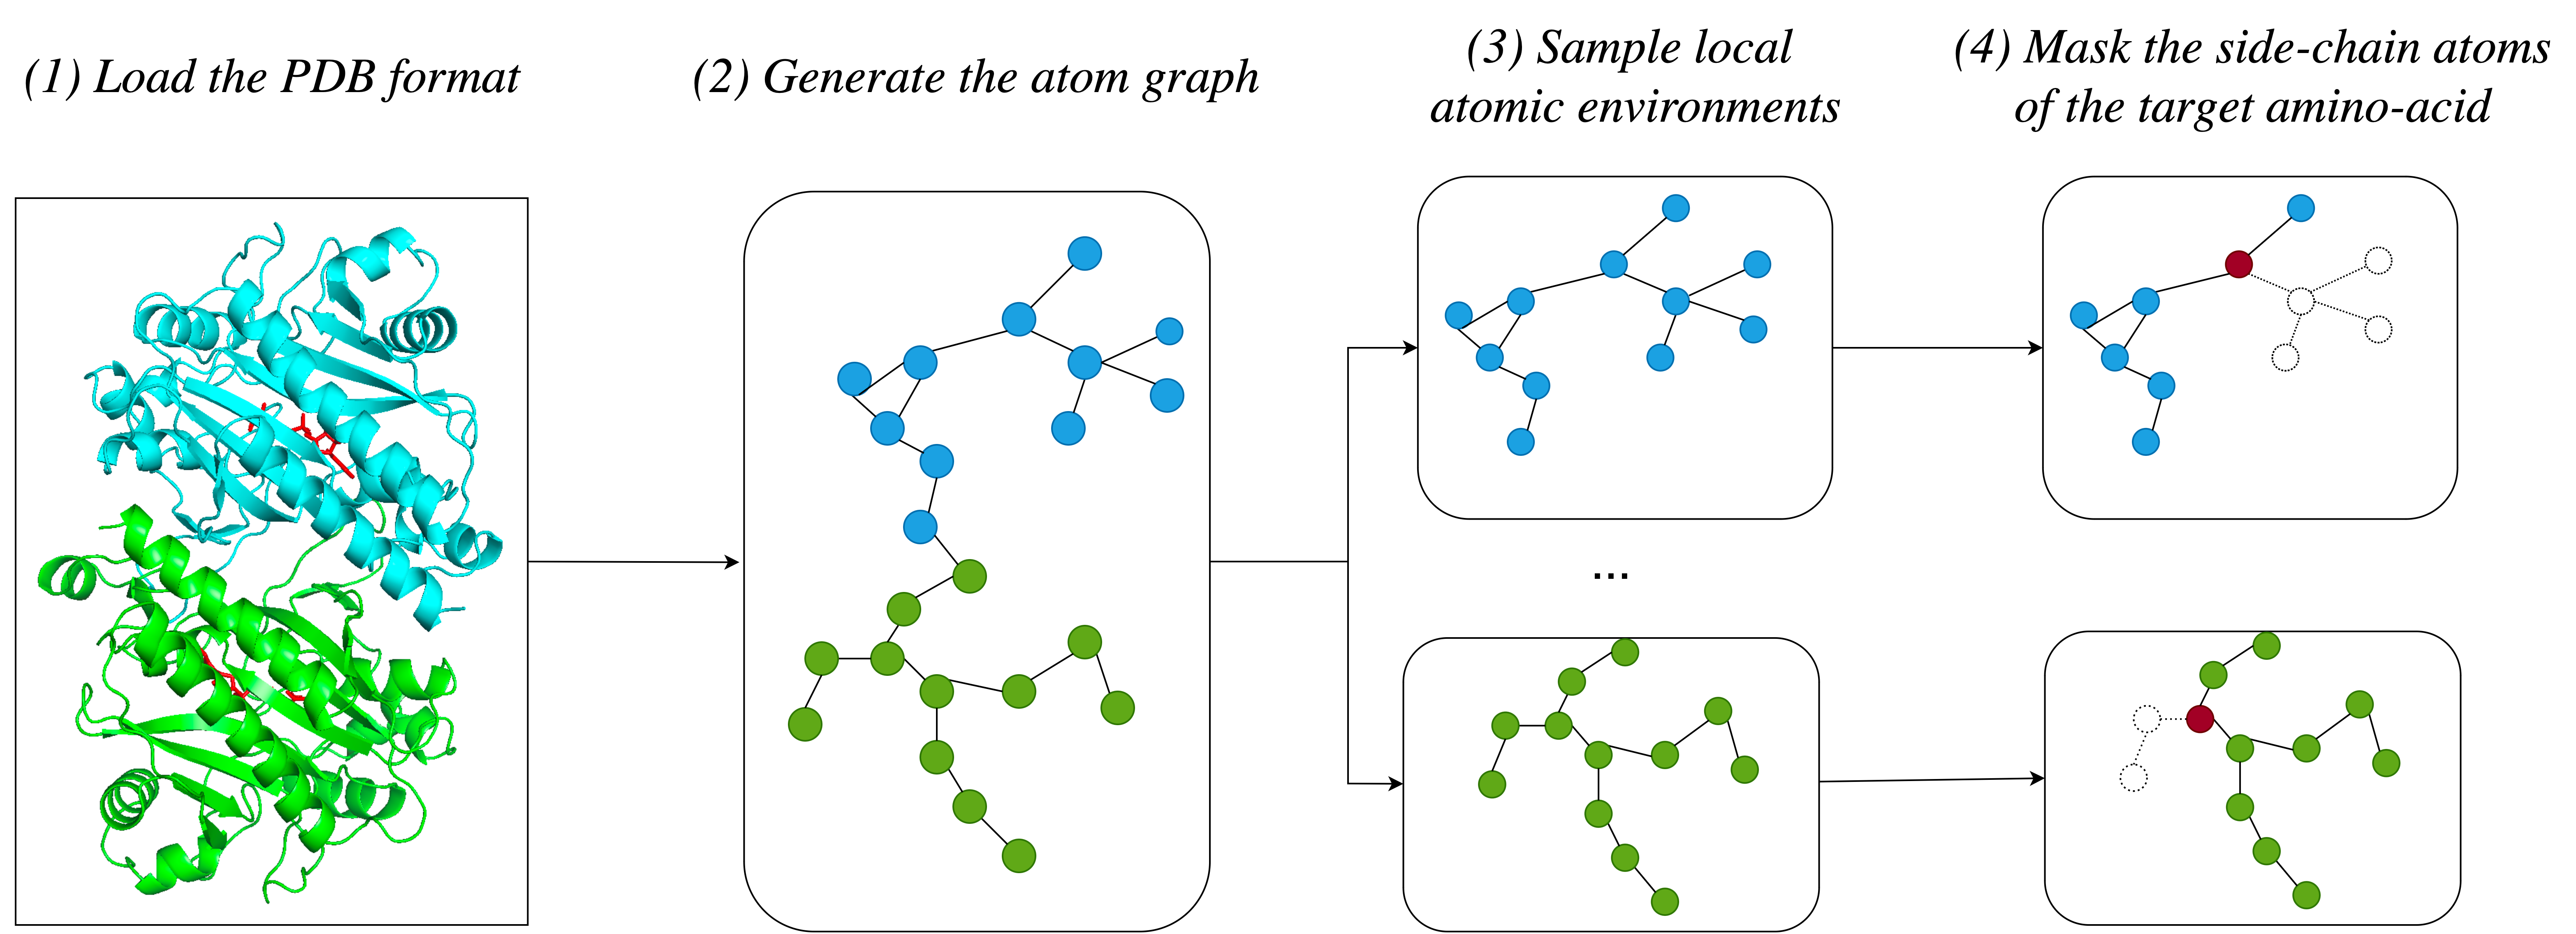
\includegraphics[width=\textwidth]{masters-report/figures/data_pipeline.png}
    \caption{Data generation pipeline for the RES task. The local atomic environments are sampled according to indices provided by the ATOM3D dataset \cite{atom-3d}. The red nodes represent the $\text{C}_{\alpha}$ carbons of their respective amino-acid residues; these are the nodes we are interested in classifying correctly.}
    \label{protein_pipeline}
\end{figure}

\begin{table}[]
    \centering
    \begin{tabular}{@{}lccc@{}}
    \toprule
    Dataset    & No. molecules & Avg no. samples/molecule & Avg no. atoms/sample \\ \midrule
    Train      & 21072           & 181                       & 622                   \\
    Validation & 962             & 199                       & 612                   \\
    Test       & 3303            & 196                       & 613                   \\ \bottomrule
    \end{tabular}
    \caption{Statistics of the ATOM3D RES dataset.}
    \label{dataset_stats}
\end{table}

\subsection{Training overview}
The training pipeline is summarised in Figure \ref{res-task}. We treat this task as a node classification task, and train the model to predict the most likely side-chain for a target $\text{C}_{\alpha}$ atom given its local environment.

\begin{figure}[!h]
    \centering
    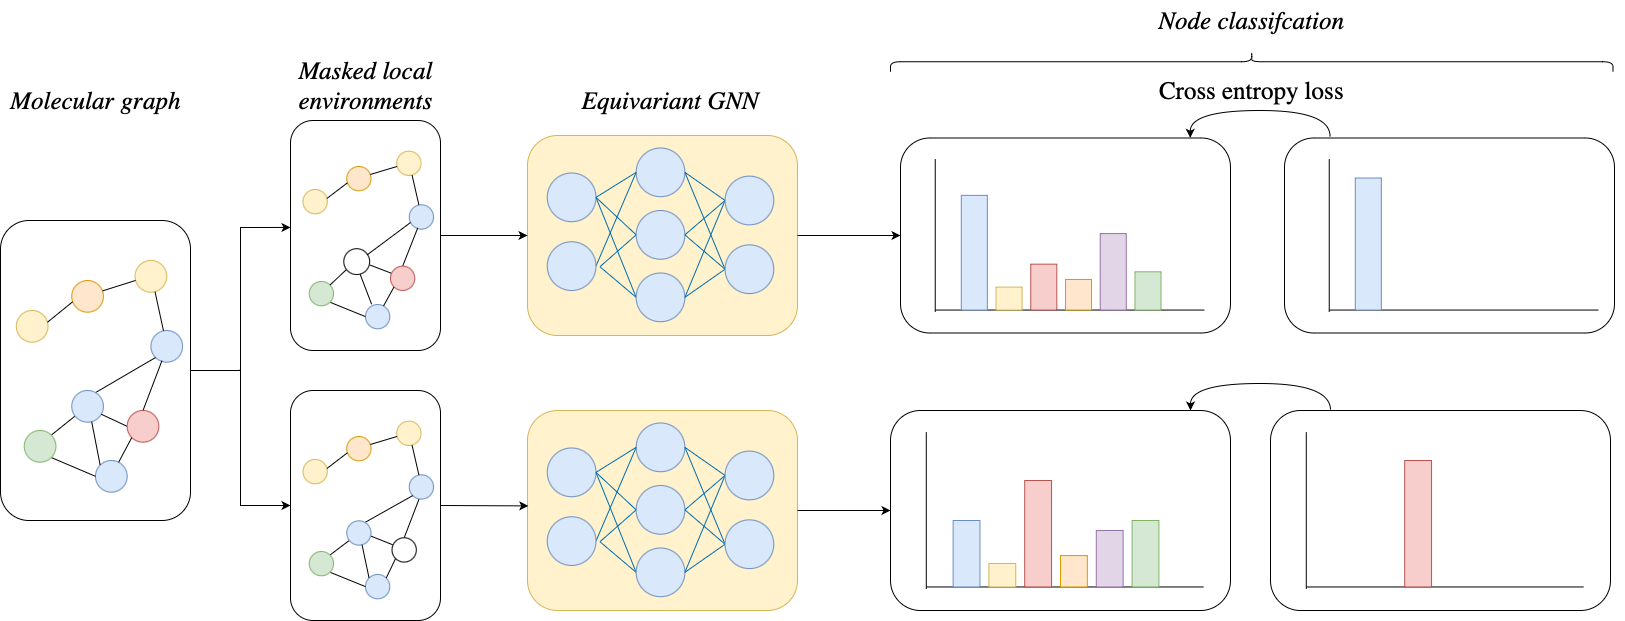
\includegraphics[width=\textwidth]{masters-report/figures/res_task_correct.png}
    \caption{Diagram of phase 1, illustrating the pipeline used in training the models on the RES task.}
    \label{res-task}
\end{figure}

\subsection{The geometric vector perceptron}
The Geometric Vector Perceptron (GVP) is an equivariant learning module first introduced by \citet{gvp1}. It lays the foundation for the GVP-GNN model, an equivariant GNN that has proven to be a successful architecture for many structure-based molecular tasks \cite{gvp1, gvp2}. In this work, we are using the second version of the GVP-GNN architecture, as described in \citet{gvp2}. 

\paragraph{The GVP module.}
The GVP module can learn both scalar-valued and vector-valued functions over geometric vectors and scalars; it can be thought of as generalising the concept of a Multi-Layer Perceptron to vectors, hence its ability to learn geometric properties of molecules. 

Borrowing some notation from \cite{gvp1}, for each node in a graph of $n$ nodes we can define the tuple $\mathbf{h} = (\mathbf{s}, \mathbf{V})$ of scalar features $\mathbf{s}\in\mathbb{R}^{n}$ and vector features $\mathbf{V}\in \mathbb{R}^{\nu\times 3}$. Then, the GVP computes updated features $\mathbf{h}'=(\mathbf{s}', \mathbf{V}') \in \mathbb{R}^m\times\mathbb{R}^{\mu \times 3}$ as can be seen in Algorithm \ref{gvp-algo}.
\begin{figure}[!h]
    \begin{minipage}[b]{0.3\textwidth}
    \centering
    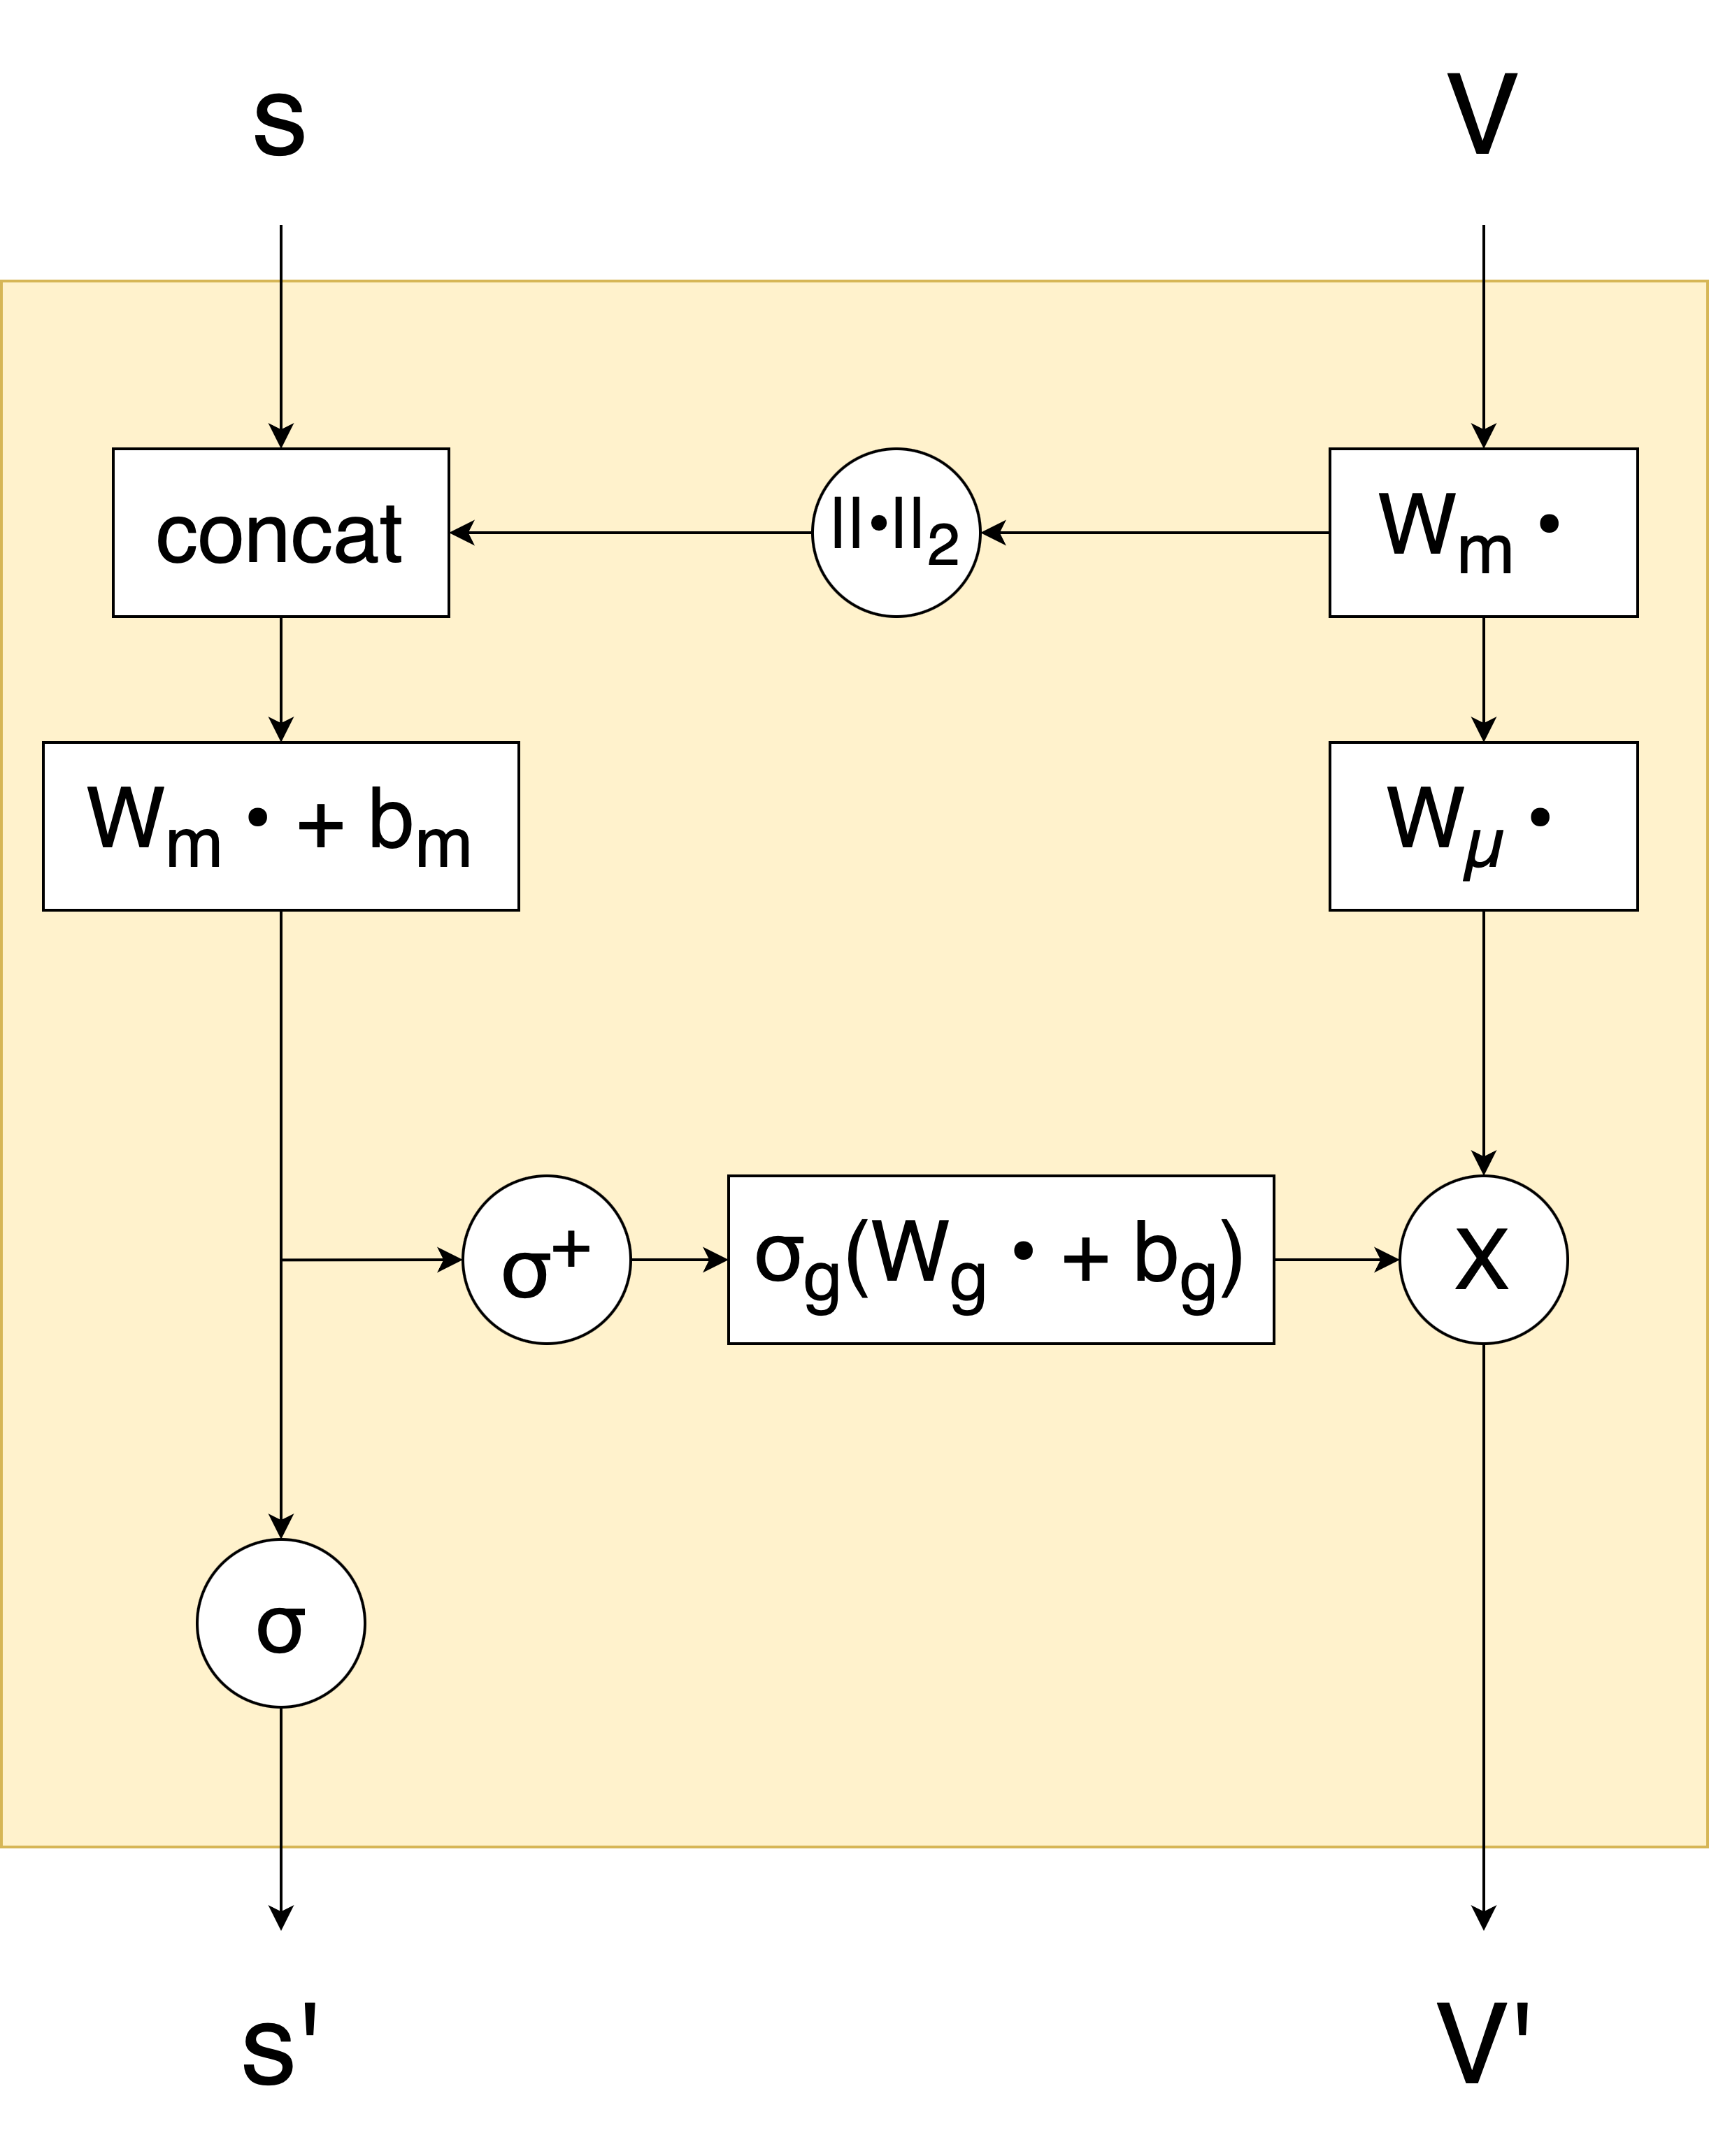
\includegraphics[width=\textwidth]{masters-report/figures/gvp.png}
    \label{fig:image}
  \end{minipage}
  \hfill
  \begin{minipage}[b]{0.65\textwidth}
    % \begin{algorithm}
% \caption{Geometric Vector Perceptron}
\hline
\begin{algorithmic}
\renewcommand{\algorithmicrequire}{\textbf{Input:}}
\renewcommand{\algorithmicensure}{\textbf{Output:}}
\Require{Scalar and vector feats. $(\mathbf{s}, \mathbf{V}) \in \mathbb{R}^n\times \mathbb{R}^{\nu \times 3}$}
\Ensure{Scalar and vector feats. $(\mathbf{s}', \mathbf{V}')\in \mathbb{R}^n\times\mathbb{R}^{\mu\times 3}$}
\State $h \gets \max(\nu, \mu)$

\State $V_h \gets \mathbf{W}_h\mathbf{V} \in \mathbb{R}^{h\times3}$

\State $V_{\mu} \gets \mathbf{W}_{\mu}\mathbf{V}_h \in \mathbb{R}^{\mu\times 3}$

\State $\mathbf{s}_h\gets ||V_h||_2$ (row-wise) $\in \mathbb{R}^h$

\State $\mathbf{v}_{\mu} \gets ||V_{\mu}||_2$ (row-wise) $\in \mathbb{R}^{\mu}$

\State $\mathbf{s}_{h + n} \gets \text{concat}(\mathbf{s}_h, \mathbf{s})\in\mathbb{R}^{h + n}$

\State $\mathbf{s}_m \gets \mathbf{W}_m\mathbf{s}_{h+n}+\mathbf{b}\in \mathbb{R}^m$

\State $\mathbf{s}' \gets \sigma(\mathbf{s}_m)\in \mathbb{R}^m $

\State $\mathbf{V}' \gets \sigma_g(\mathbf{W}_g[\sigma^{+}(\mathbf{s}_m)] + \mathbf{b}_g) \circledcirc \mathbf{V}_{\mu}$ (row-wise) $\in \mathbb{R}^{\mu \times 3}$
\\
\Return $(\mathbf{s}', \mathbf{V}')$
\end{algorithmic}
\hline
% \end{algorithm}

  \end{minipage}
\caption{\textit{(Left)} An illustration of the data flow of the module; \textit{(Right)} Algorithm showing the computation involved in a GVP module.  Both the pseudocode and the illustration are adapted from \cite{gvp2}.}
\label{gvp-algo}
\end{figure}

\paragraph{The message-passing framework.} The GVP module can be incorporated in the message-passing framework to create a \textit{GVP convolutional layer}. If $\mathbf{h}_{\mathcal{V}}^{(j)}$ are the node features of node $j$ and $\mathbf{h}_{\mathcal{E}}^{(j\rightarrow i)}$ are the edge features of edge $(j \rightarrow i)$, then the module creates the message $\mathbf{m}^{(j\rightarrow i)}$ passed from node $j$ to node $i$ as follows:
\begin{equation}
\mathbf{m}^{(j\rightarrow i)} = g_1\Big(\text{concat}(\mathbf{h}_{\mathcal{V}}^{(j)}, ~~\mathbf{h}_{\mathcal{E}}^{(j \rightarrow i)})\Big) 
\end{equation}
Assuming $k$ is the number of incoming messages, then we aggregate the messages according to:
\begin{equation}
\mathbf{m}_{\mathcal{V}}^{(i)}= \text{LayerNorm}\Big(\mathbf{h}_{\mathcal{V}}^{(i)} + \frac{1}{k}\text{Dropout}\big(\sum_{(j \rightarrow i)\in\mathcal{E}}\mathbf{m}^{(j\rightarrow i)}\big)\Big)
\label{aggregation}
\end{equation}
We follow this with a \textit{feed-forward point-wise} layer to update the node embeddings:
\begin{equation}
    \mathbf{h}_{\mathcal{V}}^{(i)}= \text{LayerNorm}\Big(\mathbf{m}_{\mathcal{V}}^{(i)} + \text{Dropout}\big(g_2(\mathbf{m}_{\mathcal{V}}^{(i)})\big)\Big)
\label{update}
\end{equation}
Functions $g_1$ and $g_2$ are compositions of three and two GVPs, respectively.

\paragraph{Layer normalisation and dropout.} Dropout \cite{dropout} is a regularisation technique that randomly ``drops out'' a portion of the neurons during training, while layer normalisation \cite{layernorm} is a technique that normalises the activations of neurons within a layer to address the problem of internal covariate shift. Both techniques are widely used in practice to avoid overfitting. 

When dealing with scalar features, the equations \ref{aggregation} and \ref{update} use the standard implementations of these two layers. However, when dealing with vector features, \citet{gvp1} modify the Dropout layer to ``drop'' entire 3D vectors. Additionally, they define layer normalisation for vector features to scale the row vectors of $\mathbf{V} =[\mathbf{v}_1, \dots, \mathbf{v}_{\nu}]$, where $\nu$ is the number of vector features per node, such that the root-mean-square norm is equal to 1: 
\begin{equation}
    \mathbf{V} \leftarrow \mathbf{V}/\sqrt{\frac{1}{\nu}||\mathbf{V}||_2^2} ~~\in \mathbb{R}^{\nu\times 3}  
\end{equation}


The final architecture is composed of GVP modules, layer normalisation modules and GVP convolutional layers, as illustrated in Figure \ref{gvp-architecture}.
\begin{figure}
    \centering
    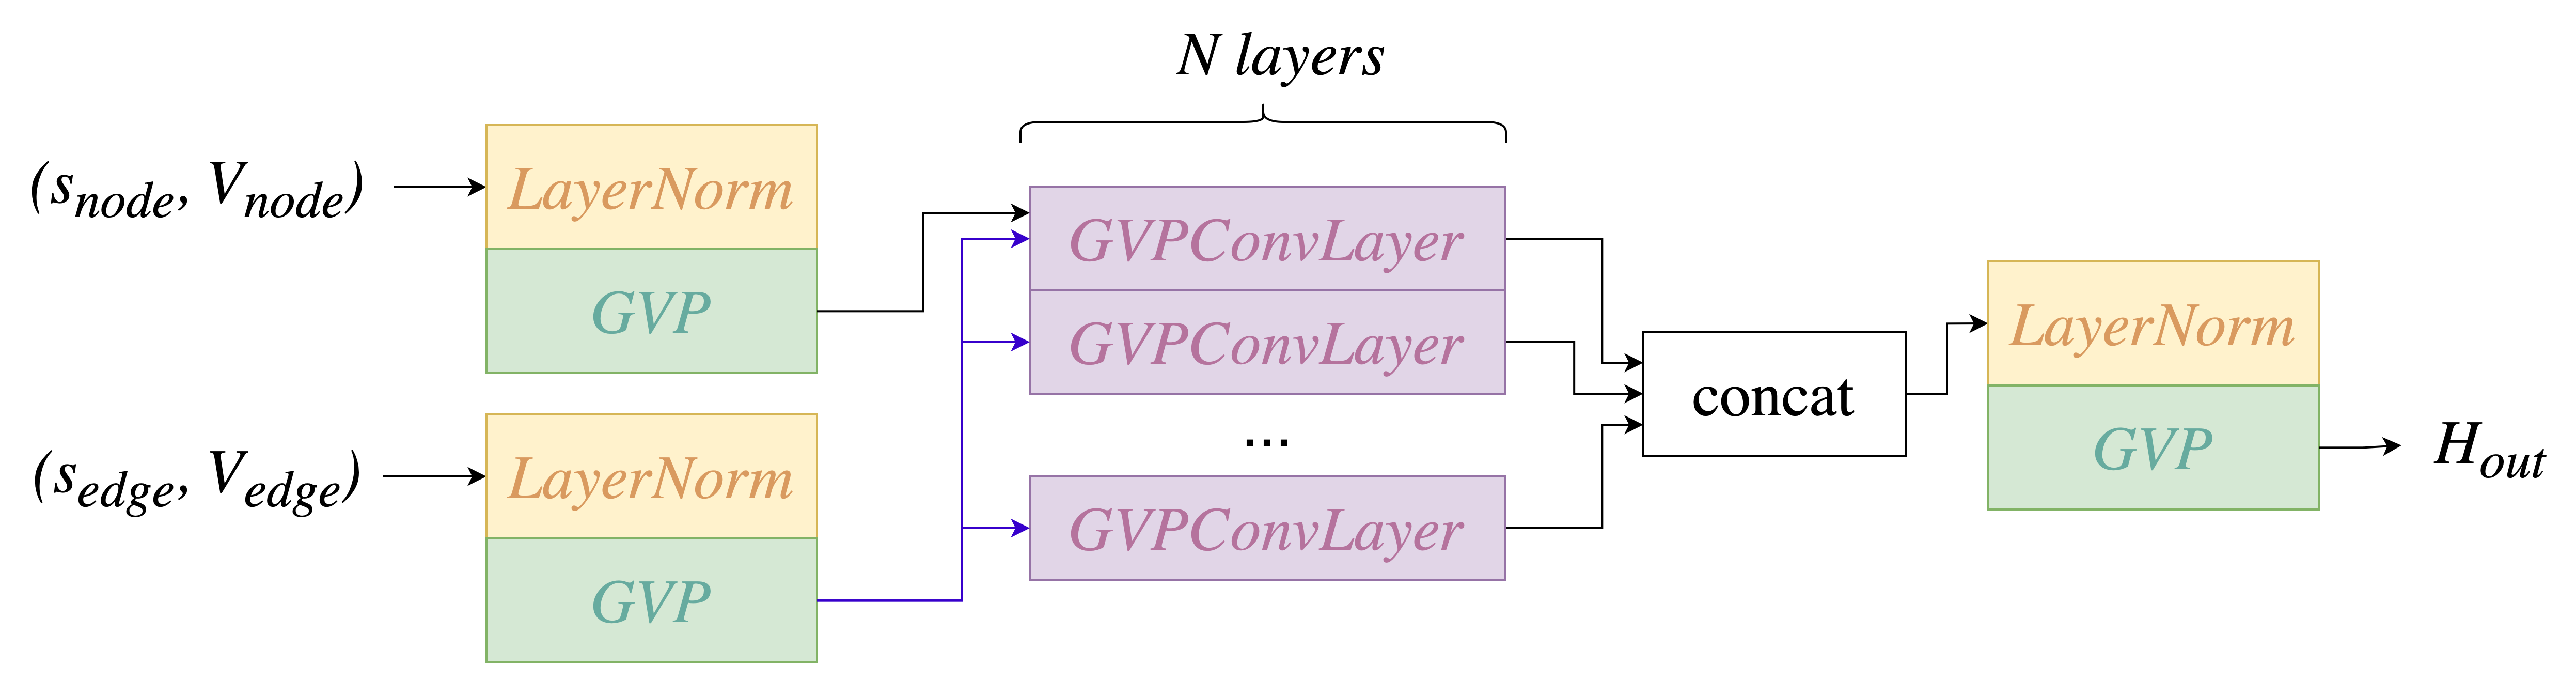
\includegraphics[width=\textwidth]{masters-report/figures/gvp_architecture_horizontal.png}
    \caption{Overall architecture of the GVP-GNN model.}
    \label{gvp-architecture}
\end{figure}

\subsection{Equivariant graph attention networks}

\subsection{The classifcation step}
\paragraph{The loss function.}
\subsection{Hyperparameters}

\section{Mutation generation}
\begin{figure}
    \centering
    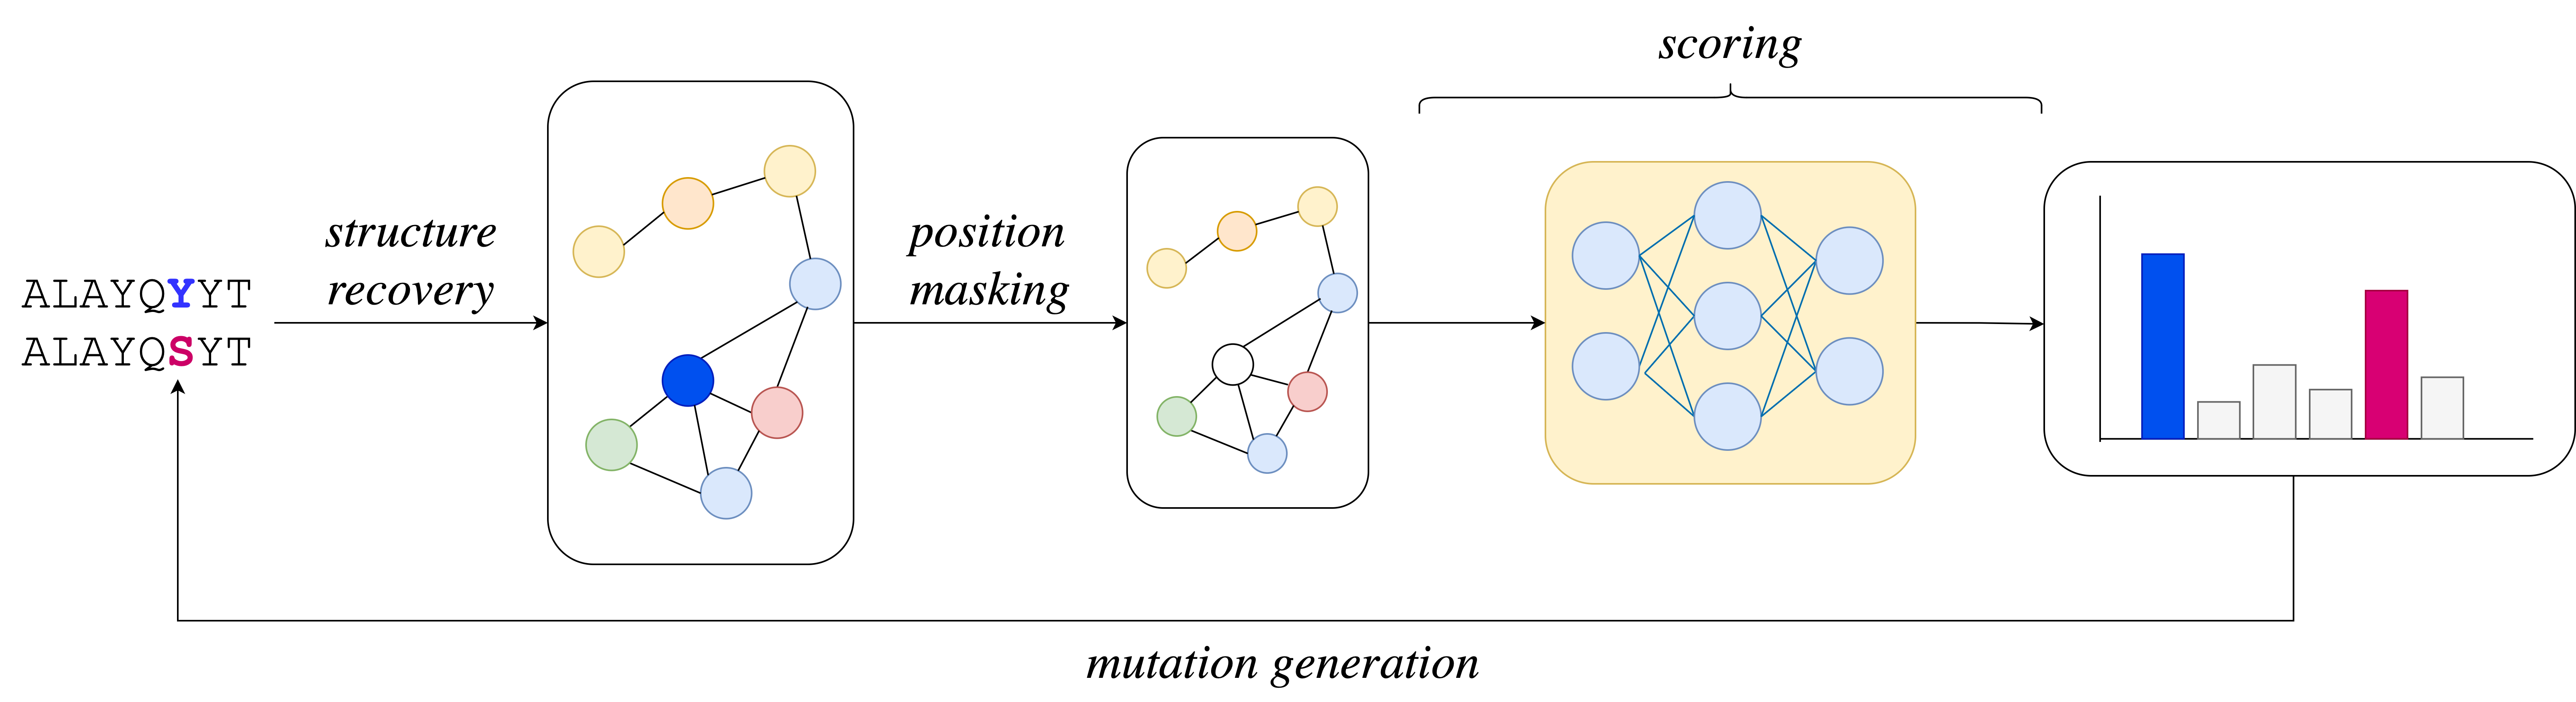
\includegraphics[width=\textwidth]{masters-report/figures/mutation_generation_2.png}
    \caption{Pipeline of phase 2.}
    \label{mutation-generation}
\end{figure}

\section{Protein fitness prediction}
\begin{figure}
    \centering
    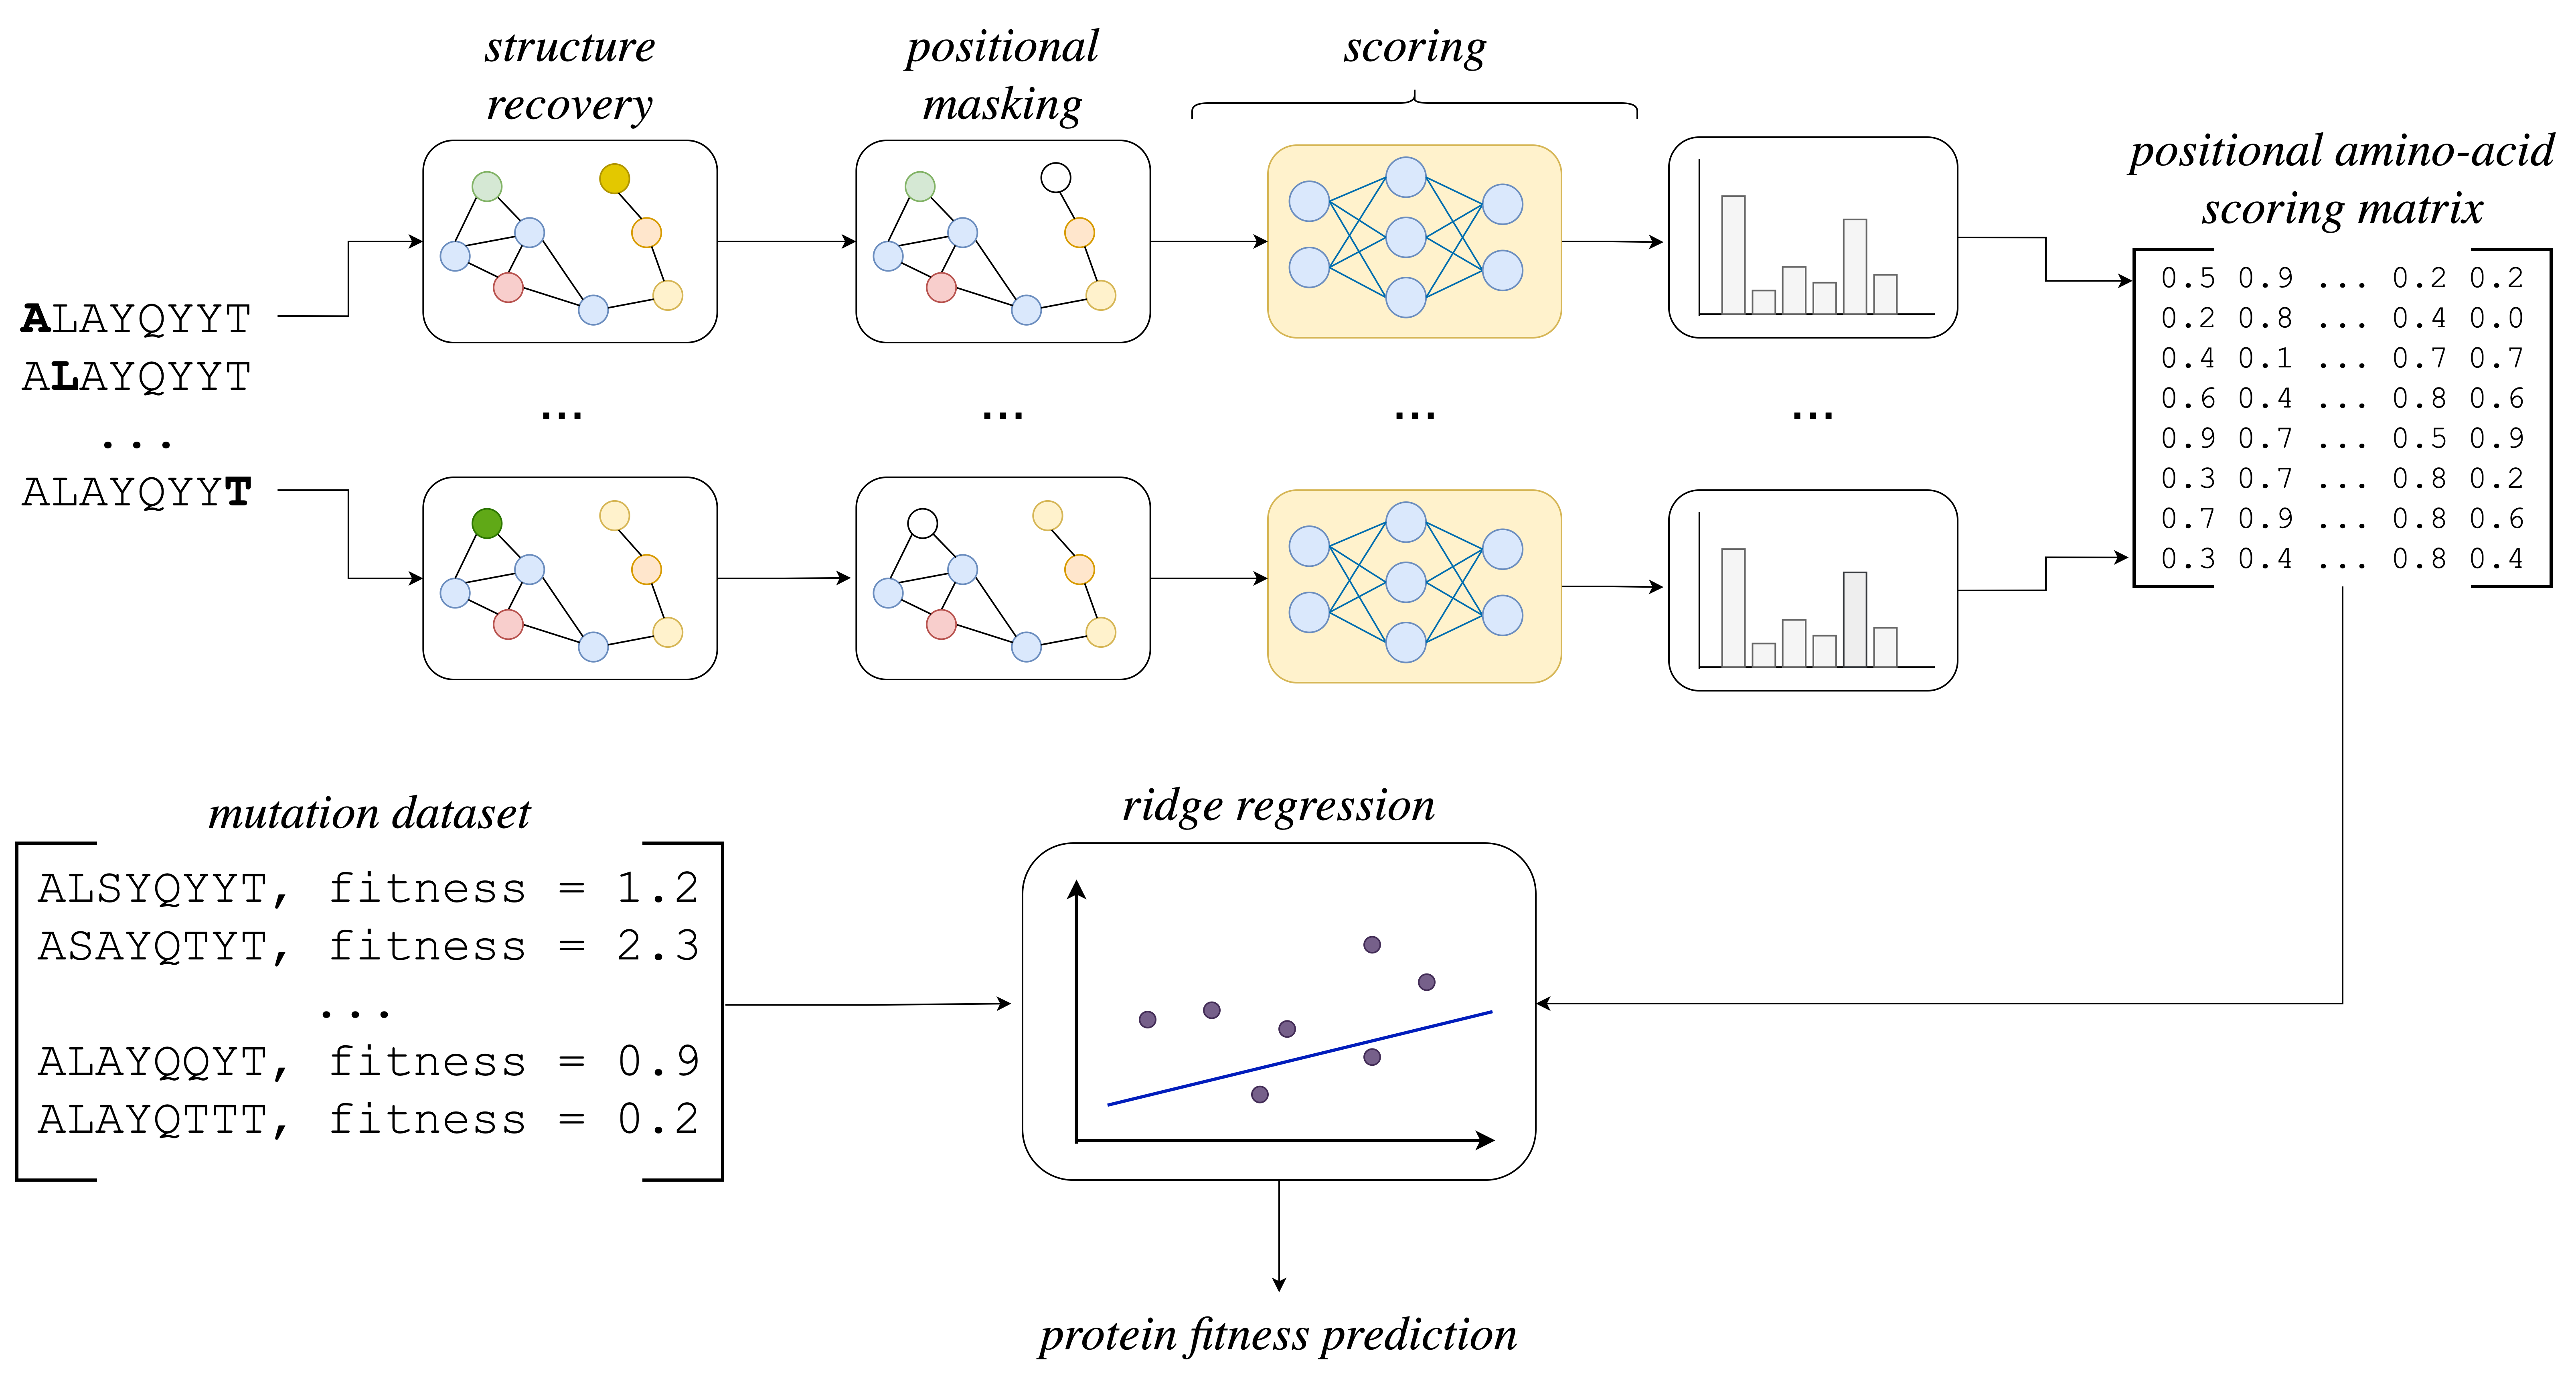
\includegraphics[width=\textwidth]{masters-report/figures/protein_fitness_prediction.png}
    \caption{Pipeline of phase 3.}
    \label{fitness-prediction}
\end{figure}
